% Options for packages loaded elsewhere
\PassOptionsToPackage{unicode}{hyperref}
\PassOptionsToPackage{hyphens}{url}
%
\documentclass[
  9pt,
]{article}
\usepackage{amsmath,amssymb}
\usepackage{lmodern}
\usepackage{iftex}
\ifPDFTeX
  \usepackage[T1]{fontenc}
  \usepackage[utf8]{inputenc}
  \usepackage{textcomp} % provide euro and other symbols
\else % if luatex or xetex
  \usepackage{unicode-math}
  \defaultfontfeatures{Scale=MatchLowercase}
  \defaultfontfeatures[\rmfamily]{Ligatures=TeX,Scale=1}
\fi
% Use upquote if available, for straight quotes in verbatim environments
\IfFileExists{upquote.sty}{\usepackage{upquote}}{}
\IfFileExists{microtype.sty}{% use microtype if available
  \usepackage[]{microtype}
  \UseMicrotypeSet[protrusion]{basicmath} % disable protrusion for tt fonts
}{}
\makeatletter
\@ifundefined{KOMAClassName}{% if non-KOMA class
  \IfFileExists{parskip.sty}{%
    \usepackage{parskip}
  }{% else
    \setlength{\parindent}{0pt}
    \setlength{\parskip}{6pt plus 2pt minus 1pt}}
}{% if KOMA class
  \KOMAoptions{parskip=half}}
\makeatother
\usepackage{xcolor}
\usepackage[margin=1in]{geometry}
\usepackage{color}
\usepackage{fancyvrb}
\newcommand{\VerbBar}{|}
\newcommand{\VERB}{\Verb[commandchars=\\\{\}]}
\DefineVerbatimEnvironment{Highlighting}{Verbatim}{commandchars=\\\{\}}
% Add ',fontsize=\small' for more characters per line
\usepackage{framed}
\definecolor{shadecolor}{RGB}{248,248,248}
\newenvironment{Shaded}{\begin{snugshade}}{\end{snugshade}}
\newcommand{\AlertTok}[1]{\textcolor[rgb]{0.94,0.16,0.16}{#1}}
\newcommand{\AnnotationTok}[1]{\textcolor[rgb]{0.56,0.35,0.01}{\textbf{\textit{#1}}}}
\newcommand{\AttributeTok}[1]{\textcolor[rgb]{0.77,0.63,0.00}{#1}}
\newcommand{\BaseNTok}[1]{\textcolor[rgb]{0.00,0.00,0.81}{#1}}
\newcommand{\BuiltInTok}[1]{#1}
\newcommand{\CharTok}[1]{\textcolor[rgb]{0.31,0.60,0.02}{#1}}
\newcommand{\CommentTok}[1]{\textcolor[rgb]{0.56,0.35,0.01}{\textit{#1}}}
\newcommand{\CommentVarTok}[1]{\textcolor[rgb]{0.56,0.35,0.01}{\textbf{\textit{#1}}}}
\newcommand{\ConstantTok}[1]{\textcolor[rgb]{0.00,0.00,0.00}{#1}}
\newcommand{\ControlFlowTok}[1]{\textcolor[rgb]{0.13,0.29,0.53}{\textbf{#1}}}
\newcommand{\DataTypeTok}[1]{\textcolor[rgb]{0.13,0.29,0.53}{#1}}
\newcommand{\DecValTok}[1]{\textcolor[rgb]{0.00,0.00,0.81}{#1}}
\newcommand{\DocumentationTok}[1]{\textcolor[rgb]{0.56,0.35,0.01}{\textbf{\textit{#1}}}}
\newcommand{\ErrorTok}[1]{\textcolor[rgb]{0.64,0.00,0.00}{\textbf{#1}}}
\newcommand{\ExtensionTok}[1]{#1}
\newcommand{\FloatTok}[1]{\textcolor[rgb]{0.00,0.00,0.81}{#1}}
\newcommand{\FunctionTok}[1]{\textcolor[rgb]{0.00,0.00,0.00}{#1}}
\newcommand{\ImportTok}[1]{#1}
\newcommand{\InformationTok}[1]{\textcolor[rgb]{0.56,0.35,0.01}{\textbf{\textit{#1}}}}
\newcommand{\KeywordTok}[1]{\textcolor[rgb]{0.13,0.29,0.53}{\textbf{#1}}}
\newcommand{\NormalTok}[1]{#1}
\newcommand{\OperatorTok}[1]{\textcolor[rgb]{0.81,0.36,0.00}{\textbf{#1}}}
\newcommand{\OtherTok}[1]{\textcolor[rgb]{0.56,0.35,0.01}{#1}}
\newcommand{\PreprocessorTok}[1]{\textcolor[rgb]{0.56,0.35,0.01}{\textit{#1}}}
\newcommand{\RegionMarkerTok}[1]{#1}
\newcommand{\SpecialCharTok}[1]{\textcolor[rgb]{0.00,0.00,0.00}{#1}}
\newcommand{\SpecialStringTok}[1]{\textcolor[rgb]{0.31,0.60,0.02}{#1}}
\newcommand{\StringTok}[1]{\textcolor[rgb]{0.31,0.60,0.02}{#1}}
\newcommand{\VariableTok}[1]{\textcolor[rgb]{0.00,0.00,0.00}{#1}}
\newcommand{\VerbatimStringTok}[1]{\textcolor[rgb]{0.31,0.60,0.02}{#1}}
\newcommand{\WarningTok}[1]{\textcolor[rgb]{0.56,0.35,0.01}{\textbf{\textit{#1}}}}
\usepackage{graphicx}
\makeatletter
\def\maxwidth{\ifdim\Gin@nat@width>\linewidth\linewidth\else\Gin@nat@width\fi}
\def\maxheight{\ifdim\Gin@nat@height>\textheight\textheight\else\Gin@nat@height\fi}
\makeatother
% Scale images if necessary, so that they will not overflow the page
% margins by default, and it is still possible to overwrite the defaults
% using explicit options in \includegraphics[width, height, ...]{}
\setkeys{Gin}{width=\maxwidth,height=\maxheight,keepaspectratio}
% Set default figure placement to htbp
\makeatletter
\def\fps@figure{htbp}
\makeatother
\setlength{\emergencystretch}{3em} % prevent overfull lines
\providecommand{\tightlist}{%
  \setlength{\itemsep}{0pt}\setlength{\parskip}{0pt}}
\setcounter{secnumdepth}{-\maxdimen} % remove section numbering
\ifLuaTeX
\usepackage[bidi=basic]{babel}
\else
\usepackage[bidi=default]{babel}
\fi
\babelprovide[main,import]{ngerman}
% get rid of language-specific shorthands (see #6817):
\let\LanguageShortHands\languageshorthands
\def\languageshorthands#1{}
\ifLuaTeX
  \usepackage{selnolig}  % disable illegal ligatures
\fi
\IfFileExists{bookmark.sty}{\usepackage{bookmark}}{\usepackage{hyperref}}
\IfFileExists{xurl.sty}{\usepackage{xurl}}{} % add URL line breaks if available
\urlstyle{same} % disable monospaced font for URLs
\hypersetup{
  pdftitle={Braunsche Molekularbewegung},
  pdfauthor={Milena Mensching, Justus Weyers},
  pdflang={de},
  hidelinks,
  pdfcreator={LaTeX via pandoc}}

\title{Braunsche Molekularbewegung}
\author{Milena Mensching, Justus Weyers}
\date{2022-12-20}

\begin{document}
\maketitle

\hypertarget{simulation}{%
\section{Simulation}\label{simulation}}

\hypertarget{experiment}{%
\section{Experiment}\label{experiment}}

\hypertarget{thema}{%
\subsection{Thema}\label{thema}}

Bestimmung dere Diffusionskonstanten eines Polystyrolpartikels, sowie
die Berechnung der Boltzmann- und Avogadrokonstanten.

\hypertarget{material}{%
\subsection{Material}\label{material}}

\begin{itemize}
\item{Mikropartikel (Polystyrol) Suspension in Wasser}
\item{Lichtmikroskop mit Objektträger}
\item{Deckplättchen}
\item{Thermometer}
\item{Zur Messung und Auswertung wurden folgende Computerprogramme benutzt: ThorCam, Tracker, SciDAVis, Python, R.}
\end{itemize}

\hypertarget{versuchsaufbau-und-durchfuxfchrung}{%
\subsection{Versuchsaufbau und
Durchführung}\label{versuchsaufbau-und-durchfuxfchrung}}

\begin{figure}
\centering
\includegraphics[width=\textwidth,height=0.2\textheight]{Bilder/Objektträger.png}
\caption{Mikroskop mit Probe}
\end{figure}

Auf einen Objektträger wurde ein Tropfen einer Mikropartikel
(Polystyrol) Suspension in Wasser gegeben. Zwei Deckplättchen wurden
neben den Tropfen, und eines mittig auf die anderen beiden positioniert
und unter das Mikroskop gelegt. Die Polystyrolpartikel (PSP) wurden
scharf gestellt. Als Vergrößerung wurde 40/0.65 gewählt.

\hypertarget{durchfuxfchrung}{%
\subsection{Durchführung}\label{durchfuxfchrung}}

Mit Hilfe einer Mikroskopkamera und des Programms ``ThorCam'' wird die
Projektion auf dem Bildschirm sichtbar. Eine Zeitreihe über den Zeitraum
von hundert Sekunden und im Umfang von 100 Bildern wurde von den PSP
automatisch, mittels ``ThorCam'', erstellt.

Nach Aufnehmen der Messreihe wurde die Temperatur gemessen. Diese betrug
21,7°C. Danach wurde mit Hilfe des Programms ``Tracker'' die Position
des Teilchens ausgewertet. Dafür wird in einem Datensatz von 100 Bildern
das ``Teilchen of interest'' mit dem Cursor markiert.

Nachdem sich die Verarbeitung der Daten als kompliziert herausgestellt
hatte, wurde abweichend von erster Methode eine zweite Auswertung des
Bildmaterials vorgenommen. Diese bestand darin, mittels eines Programmes
die Mittelpunkte aller 17 PSP in allen 100 Einzelbildern zu bestimmen.
Das verwendete Pythonscript umfasste eine Schwarz-Weiß-Maskierung der
Einzelbilder und eine Clusterung. Der Mittelpunkt jedes PSP wurden als
Mittelpunkt aller zugehörigen Bildpixel in Bildkoordinaten berechnet und
im Zeitverlauf als csv-Datei gespeichert.

\hypertarget{fehlerbetrachtung}{%
\subsection{Fehlerbetrachtung}\label{fehlerbetrachtung}}

Eine Unsicherheit der Methodik besteht in der Umrechnung der Bildpunkte
in Meter. Eine zweite Unsicherheit besteht in der Auflösung des Bildes.
Eine dritte Unsicherheit besteht in dem verwendeten Programm. Letztere
Unsicherheit wird aber als kleiner eingeschätzt, als die manuelle
Auswertung.

\hypertarget{beobachtungen}{%
\subsection{Beobachtungen}\label{beobachtungen}}

Zu Beginn werden die zurückglegten Wege aller PSP im Bildausschnitt
geplottet. Ein einzelner, ausgewählter Partikel (NR. 2) wird
exemplarisch genauer dargestellt, indem dessen Bewegungspfad einzeln in
einem höheren Maßstab geplottet wird.

\begin{figure}
\centering
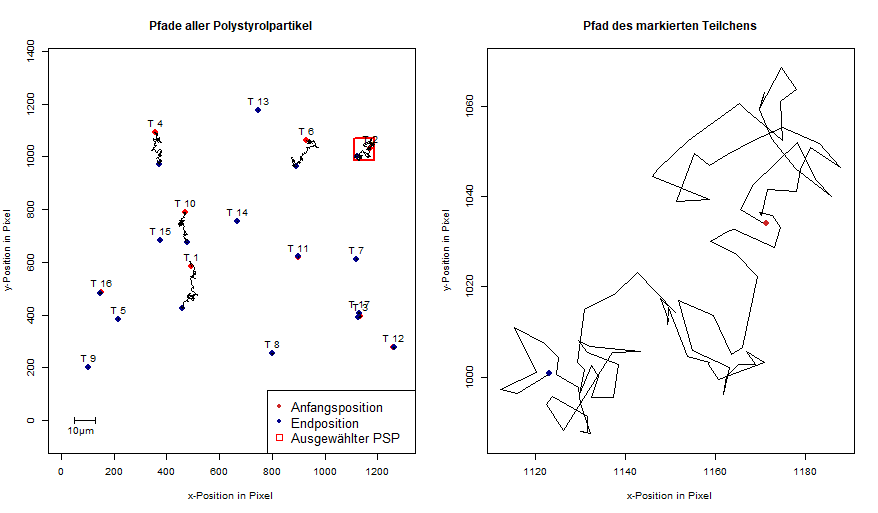
\includegraphics[width=\textwidth,height=0.2\textheight]{code/Plots/Raum.png}
\caption{Auf diesen zwei Plots sind die Positionen aller bzw. eines
markierten PSP im zeitlichen Verlauf zu sehen. Die Aufnahmedauer betrug
100 s mit 1 fps. Die PSP wurden zudem nummeriert.}
\end{figure}

Auf Abbildung 2 ist erkennbar, dass die 17 beobachteten PSP sich in
ihren zurückgelegten Wegen deutlich unterscheiden. Während 12 PSP sich
praktisch nicht von ihrer Ausgangsposition bewegt haben, ist bei sechs
Teilchen eine deutliche Abweichung zwischen Anfangs- und Endposition
auszumachen. Es ist nicht verwunderlich, dass viele Partikel keinen
räumlichen Versatz aufweisen. Netto sollte die Bewegung aller
Randomwalks zusammengenommen zu einem Verharren jedes Teilchens an
seinem Ursprung führen, Abweichungen durch die Standardabweichungen sind
möglich. Andere Erklärungen, wie die Ortsgebundenheit als Folge von
adhäsiven Kräften zwischen PSP und den Glasplättchen sind aber auch
denkbar. Zwar sind auch für die scheinbar unbewegten Teilchen Bewegungen
bestimmt worden, diese sind aber mikroskopisch kaum nachweisbar und
könnten ein Resultat der Unsicherheit beim verwendeten visuellen
Messverfahren sein.

Interpretationsspielraum geben die zurückgelegten Pfade der fünf anderen
Teilchen (T 1, 2, 4, 6, 10, siehe Abbildung 2). Diese weisen trotz aller
Zufälligkeit der einzelnen random-walks eine gewisse Tendenz zu einer
Bewegung entgegen der y-Achse auf. Hier stellt such die Frage, ob neben
der diffusiven Bewegungskomponente auch eine advektive
Transportkomponente einen Einfluss auf die Teilchenbewegung hat. Dies
würde insofern gut den Sachverhalt erklären, als dass eine zufällige,
diffusive Bewegungskomponente und eine der y-Achse entgegengerichteten,
advektiven Hauptbewegungskomponente zusammengenommen, für ein Ensemble
von Teilchen solche Bewegungspfaden bewirken würde. Ursache könnte eine
kleine Strömung auf mikroskopischer Ebene zwischen den Glasplättchen
sein, möglicherweise verursacht durch einen Temperaturgradienten
aufgrund der erhöhten Temperatur des Wassers im Lichtgang des
Mikroskopes.

\hypertarget{umrechnung-der-messwerte-in-meter}{%
\subsubsection{Umrechnung der Messwerte in
Meter}\label{umrechnung-der-messwerte-in-meter}}

Im nächsten Schritt können die ermittelten Werte für die Diffusionspfade
von Pixel in Meter umgerechnet werden. Dafür ist der Maßstab der
aufgenommenen Bilder vonnöten. Dafür werden die PSP selbst verwendet,
von denen bekannt ist, dass deren Durchmesser 2µm beträgt. Beim Zählen
der Pixel ist darauf geachtet worden, die Originalauflösung zu
verwenden, in der auch die Berechnung der Schrittweiten berechnet wurde.

\begin{figure}
\centering
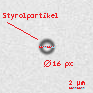
\includegraphics[width=\textwidth,height=0.21\textheight]{Bilder/styrolpartikel.png}
\caption{Polystyrolpartikel mit dem Durchmesser 2µm. Der Durchmesser ist
in Pixel abgemessen und beträgt 16 Pixel.}
\end{figure}

Aus dem Zusammenhang, dass sechzehn Bildpixel zwei Mikrometern
entsprechen, folgt für die Kantenlänge eines Pixels eine Länge von
\(0,125 \mu m\). Die kleinste ablesbare Skala in dem Bild ist der
Durchmesser von \(2\mu m\) des PSP. Für die Unsicherheit der Kantenlänge
eines Pixels folgt so
\(u_{Pixellänge} = \frac{1}{16}\cdot \frac{2\mu m}{2\sqrt{6}} = 0,026\mu m\).

\begin{Shaded}
\begin{Highlighting}[]
\CommentTok{\# Berechnung der Kantenlänge eines Pixels}
\DecValTok{2}\SpecialCharTok{*}\DecValTok{10}\SpecialCharTok{**}\NormalTok{(}\SpecialCharTok{{-}}\DecValTok{6}\NormalTok{)}\SpecialCharTok{/}\DecValTok{16}
\end{Highlighting}
\end{Shaded}

\begin{verbatim}
## [1] 1.25e-07
\end{verbatim}

\begin{Shaded}
\begin{Highlighting}[]
\CommentTok{\# Berechnung Unsicherheit der Kantenlänge:}
\DecValTok{2}\SpecialCharTok{*}\DecValTok{10}\SpecialCharTok{**}\NormalTok{(}\SpecialCharTok{{-}}\DecValTok{6}\NormalTok{)}\SpecialCharTok{/}\NormalTok{(}\DecValTok{16}\SpecialCharTok{*}\DecValTok{2}\SpecialCharTok{*}\FunctionTok{sqrt}\NormalTok{(}\DecValTok{6}\NormalTok{))}
\end{Highlighting}
\end{Shaded}

\begin{verbatim}
## [1] 2.551552e-08
\end{verbatim}

\hypertarget{statistische-untersuchung}{%
\subsubsection{Statistische
Untersuchung}\label{statistische-untersuchung}}

Nach dieser Umrechnung kann mit statistischen Mitteln versucht werden,
weitere Aussagen über das Diffusionsverhalten der PSP zu treffen. Dazu
werden verschiedene Histogramme erstellt, die folgende Bewegungen, der
in Abbildung 2 nummerierten Teilchen Erfassen:

\begin{itemize}
\item Bewegung von Teilchen 2
\item Bewegung der viel bewegten Teilchen (Teilchen 1, 2, 4, 6, 10)
\item Bewegung der wenig bewegten Teilchen (Teilchen 3, 5, 7, 8, 9, 11, 12, 13, 14, 15, 16, 17)
\item Bewegung aller Teilchen
\end{itemize}

Untersucht werden die Schrittweiten in x und y Richtung, deren Betrag
über den Satz des Pythagoras berechnet wurde.

\begin{figure}
\centering
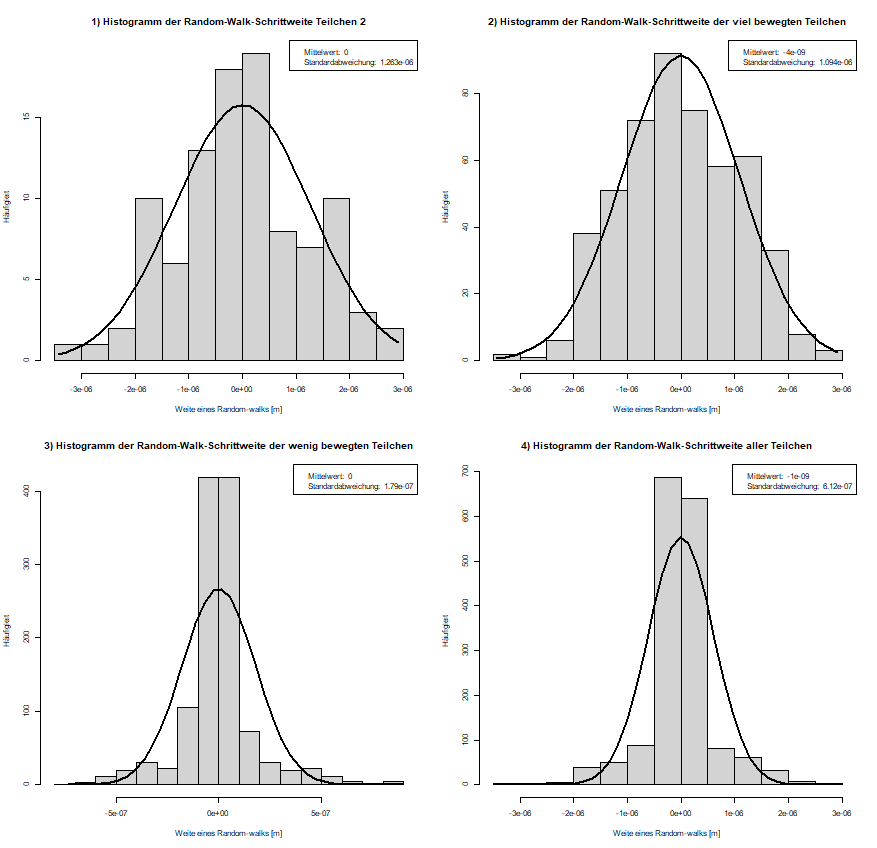
\includegraphics[width=\textwidth,height=0.31\textheight]{code/Plots/Hist.png}
\caption{Die vier Histogramme zeigen die Häufigkeit der Schrittweiten
pro Random-walk für vier verschiedene Gruppen von Teilchen}
\end{figure}

Die Histogramme sehen eigentlich alle ganz gut normalverteilt aus.
Unterschiede in der Standardabweichung sind zwischen den wenig und den
viel bewegten Teilchen erkennbar, bei letzteren ist die
Standardabweichung um \(0,45\mu m\) größer. Die Mittelwerte aller
Verteilungen liegen, wie erwartbar, allesamt praktisch bei Null.

\hypertarget{auswertung}{%
\subsection{Auswertung}\label{auswertung}}

Mittels der folgender Formel kann für jedes Teilchen die zugehörige
Diffusionskonstante \(D\) berechnet werden: \[D=\frac{\sigma^2}{2t}\]
Mit:

\begin{itemize}
\item $\sigma$: Standardabweichung der Schrittweite eines Random-walks für ein PSP
\item $t$: Zeitintervall zwischen zwei Bildaufnahmen ($t=1s=const.$).
\end{itemize}

\hypertarget{berechnung-der-diffusionskonstante}{%
\subsubsection{Berechnung der
Diffusionskonstante}\label{berechnung-der-diffusionskonstante}}

\hypertarget{interpretation}{%
\subsection{Interpretation}\label{interpretation}}

\end{document}
